\documentclass[tikz]{standalone}

% Required packages
\usepackage[utf8]{inputenc}
\usepackage[T1]{fontenc}
\usepackage{lmodern} % For smooth fonts
\usepackage{amsmath} % For math symbols like \forall and \in
\usepackage{tikz}

% TikZ libraries for advanced features
\usetikzlibrary{
    positioning,      % For placing nodes relative to each other (e.g., right=of)
    decorations.pathreplacing, % For drawing curly braces
    arrows.meta,      % For modern arrow tips (e.g., Stealth)
    calc              % For calculating coordinates (e.g., midpoints)
}

\begin{document}
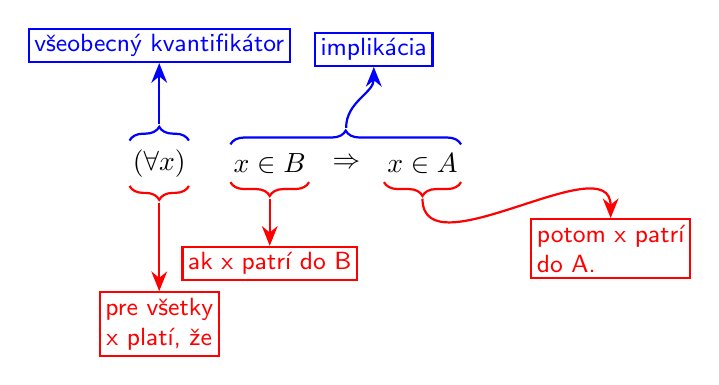
\begin{tikzpicture}[
    % Global style settings
    node distance=0.8em and 1.5em, % Default vertical and horizontal spacing for nodes
    % Style for the blue elements
    blue_style/.style={
        color=blue, 
        thick
    },
    % Style for the red elements
    red_style/.style={
        color=red, 
        thick
    },
    % Style for arrowheads
    arrow_tip/.style={
        -{Stealth[length=2.5mm, width=2mm]}
    },
    % Style for the text labels (smaller font, boxed)
    label_style/.style={
        draw, % This adds the box around the node
        font=\sffamily\small, % Use a small, sans-serif font
        inner sep=2pt % Add a little padding inside the box
    }
]
    % 1. Define the nodes for the main formula.
    \node[inner sep=1pt] (quantifier) {$(\forall x)$};
    \node[inner sep=1pt, right=of quantifier] (set_b) {$x \in B$};
    \node[right=0.5em of set_b] (implies) {$\Rightarrow$};
    \node[inner sep=1pt, right=0.5em of implies] (set_a) {$x \in A$};

    % 2. Place the annotation text nodes.
    \node[blue_style, label_style, above=3em of quantifier] (quant_text_up) {všeobecný kvantifikátor};
    \coordinate (implication_midpoint) at ($(set_b.north)!0.5!(set_a.north)$);
    \node[blue_style, label_style, above=3em of implication_midpoint, xshift=1em] (impl_text_up) {implikácia}; 

    \node[red_style, label_style, below=4em of quantifier, align=center] (quant_text_down) {pre všetky \\ x platí, že};
    \node[red_style, label_style, below=2.5em of set_b] (b_text_down) {ak x patrí do B};
    \node[red_style, label_style, below right=1.5em and 2.5em of set_a, align=left] (a_text_down) {potom x patrí \\ do A.};

    % 3. Draw the decorative curly braces (blue down, red up).
    \draw[blue_style, decorate, decoration={brace, amplitude=5pt, raise=2pt}]
        (quantifier.north west) -- (quantifier.north east);
    \draw[blue_style, decorate, decoration={brace, amplitude=5pt, raise=2pt}]
        (set_b.north west) -- (set_a.north east);

    \draw[red_style, decorate, decoration={brace, amplitude=5pt, mirror, raise=2pt}]
        (quantifier.south west) -- (quantifier.south east);
    \draw[red_style, decorate, decoration={brace, amplitude=5pt, mirror, raise=2pt}]
        (set_b.south west) -- (set_b.south east);
    \draw[red_style, decorate, decoration={brace, amplitude=5pt, mirror, raise=2pt}]
        (set_a.south west) -- (set_a.south east);

    % 4. Draw the arrows with the new double-bend curvy style.
    % --- Blue arrows (up)
    % 'out=90' leaves vertically up, 'in=-90' arrives vertically from above.
    \draw[blue_style, arrow_tip] ($(quantifier.north)+(0,8pt)$) to[out=90, in=-90] (quant_text_up.south);
    \draw[blue_style, arrow_tip] ($(implication_midpoint)+(0,8pt)$) to[out=90, in=-90] (impl_text_up.south);

    % --- Red arrows (down)
    % 'out=-90' leaves vertically down, 'in=90' arrives vertically from below.
    \draw[red_style, arrow_tip] ($(quantifier.south)-(0,8pt)$) to[out=-90, in=90] (quant_text_down.north);
    \draw[red_style, arrow_tip] ($(set_b.south)-(0,8pt)$) to[out=-90, in=90] (b_text_down.north);
    \draw[red_style, arrow_tip] ($(set_a.south)-(0,8pt)$) to[out=-90, in=90] (a_text_down.north);

\end{tikzpicture}
\end{document}
